\documentclass[12pt]{article}
\usepackage[spanish]{babel}
\usepackage[utf8]{inputenc}
\usepackage{graphicx}
\usepackage{wrapfig}
\usepackage{hyperref}



\begin{document}


	
\begin{titlepage}
\centering
{\bfseries\LARGE Universidad Nacional de La Plata \par}
\vspace{1cm}
{\scshape\Large Facultad de Informática \par}
\vspace{3cm}
{\scshape\Huge ScrabbleAR \par}
\vfill
{\Large Autores: \par}
{\Large Juan Sebastián Peña,  Hernán Nahuel Ramos, Felipe Verdugo \par}
\vfill
{\Large Julio 2020 \par}
\end{titlepage}




\tableofcontents

\section{Introducción}

En este informe se detalla el proceso de implementación del juego denominado ScrabbleAR desarrollado en la materia Seminario de Lenguajes de Python.

Debido a que es un trabajo integrador, se aplicaron todos los conocimientos adquiridos durante la cursada y a su vez este trabajo requirió implementar una coordinación entre los estudiantes que realizaron dicho trabajo para poder dividir tareas (la comunicación entre los integrantes es muy importante en lo mencionado anteriormente)

A continuación, se va a detallar y explicar que módulos se utilizaron, reglas del juego, problemas que surgieron durante el desarrollo, guías y etc.


\section{Reglas}
\label{sec:reglas}
\subsection{Generales}
El jugador debe formar una palabra usando dos (2) o más letras, colocándolas horizontalmente (las letras ubicadas de izquierda a derecha) o verticalmente (en orden descendente) sobre el tablero. En la primera jugada, una de las letras deberá estar situada en el cuadro de “inicio del juego”.

Para comenzar la partida, cada jugador retira siete (7) fichas de la bolsa. Luego combina dos o más de sus letras para formar una palabra, y la coloca en el tablero horizontal o verticalmente. Está obligado a poner una de las letras que forman su palabra en la casilla central.

Una vez ingresada la palabra se debería confirmar la misma en el tablero y automáticamente se chequeará si la palabra corresponde a la clasificación que se está usando en el juego. Las únicas palabras admitidas en el tablero serán adjetivos, sustantivos y verbos, de acuerdo a las opciones de configuración establecidas previamente. En caso de no corresponder, las fichas serán devueltas al jugador para que vuelva a intentar.

Una vez que el jugador haya ingresado y confirmado correctamente la palabra, se le repondrá la cantidad de fichas que utilizó sin contar las preexistentes en el tablero. De esta manera el jugador nunca tendrá más de siete (7) fichas en su poder.

Cuando el turno lo tiene la computadora, se tratará de armar palabras con las fichas propias de la computadora. La primera combinación que concuerde es la que se tomará como válida. En caso de no encontrar combinación, pasará su turno.

En cualquier momento del juego, el jugador puede decidir usar un turno para cambiar algunas o todas sus fichas, devolviéndolas a la bolsa de fichas del juego y reemplazándolas por la misma cantidad; al final, siempre debe tener siete (7). En este mismo turno, el jugador no podrá colocar ninguna palabra sobre el tablero. Esta opción no está disponible para la computadora y el jugador sólo podrá usarla como máximo tres veces durante el juego.

\subsection{Atril}
  Hay dos atriles uno para el usuario y otro para la computadora.
  
  El atril de cada usuario tiene siete letras.
  
  Cada usuario, incluyendo la computadora, tiene tres posibilidades de cambiar su atril de letras.


\subsection{Tablero}

\
\


Hay tres tableros de dimensión 15x15, con dificultades diferentes según el nivel que se elija (fácil, medio, difícil).

\
\
\
\newpage

Fácil: se incluyen casilleros con más premios para duplicar y triplicar el valor de palabra y letra y no cuenta con casilleros que restan 3 puntos.
\newline
\newline
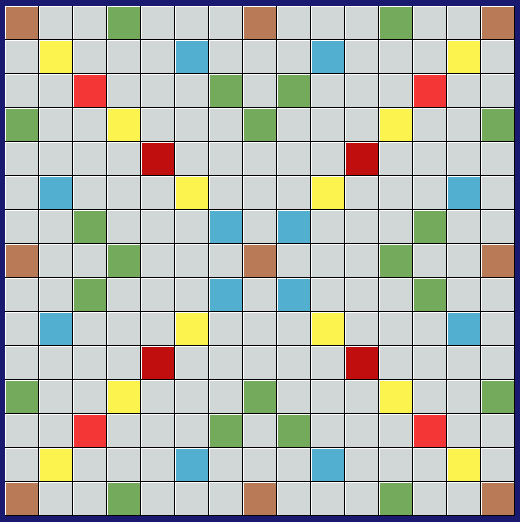
\includegraphics[width=\textwidth]{images/facil.png}

\
\
\
\newpage
Medio: es igual al tablero "fácil" pero en este caso se incluyen casilleros que restan 3 puntos.
\newline
\newline
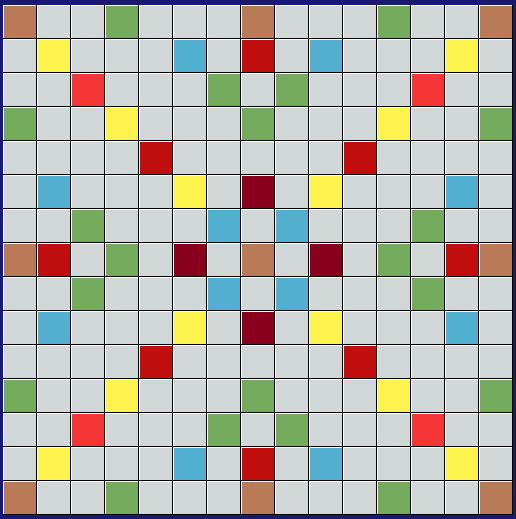
\includegraphics[width=\textwidth]{images/medio.png}
\
\
\
\newpage
Difícil: se incluyeron menos casilleros que duplican y triplican, y se agregan más que restan 3 puntos.
\newline
\newline
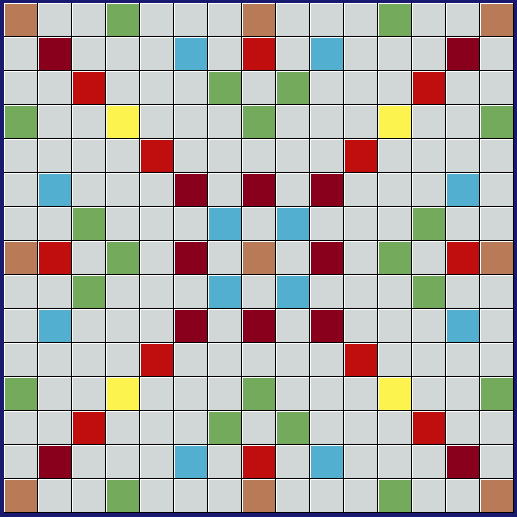
\includegraphics[width=\textwidth]{images/dificil.png}

\subsection{Letras}
La bolsa de las letras tiene 98 letras.
Cada palabra tiene su propio puntaje y cantidad de letras.
   
   
\subsection{Tiempo de juego}       

 Tiempo de juego: se configurará un máximo de tiempo para una partida de
 acuerdo a cada nivel.
 En este caso, se contará con la opción de elegir un tiempo de 20, 40 o 60 minutos.
 
\subsection{Nivel}
Se proponen tres niveles de dificultad: fácil, medio y difícil. Esto condiciona el tiempo y el conjunto de palabras disponibles.
En el nivel fácil, se puede jugar con cualquier tipo de palabra (adjetivos, sustantivos y verbos); en el nivel medio, se juega sólo con verbos y sustantivos y en el nivel difícil con una categoría al azar. En esta opción, se configurará el nivel del juego.


\subsection{Puntaje}
 El puntaje de cada ficha:
 
 1 punto: A, E, O, S, I, U, N, L, R, T

 2 puntos: C, D, G

 3 puntos: M, B, P

 4 puntos: F, H, V, Y

 6 puntos: J

 8 puntos: K, Q, W, X

 10 puntos: Z

Igualmente, el puntaje de cada ficha puede ser configurable.

\subsection{Fichas}

La cantidad total de fichas por letra. esta configuración será la misma para todos los niveles:

 A x 11, E x 11, O x 8, S x 7, I x 6, U x 6, N x 5, L x 4, R x 4, T x 4
    
 C x 4, D x 4, G x 2
    
 M x 3, B x 3, P x 2
    
 F x 2, H x 2, V x 2, Y x 1
    
 J x 2
    
 K x 1, Q x 1, W x 1, X x 1
    
 Z x 1

Igualmente, la cantidad de fichas se puede configurar en Opciones avanzadas.

\subsection{Premio por letra}


Casillas con premio para letras: al colocar una ficha en una casilla celeste (triplica letra), se triplica   el valor de dicha letra; y al colocarla en una casilla marrón (doble de letra), se duplica su valor.
 
\subsection{Premio por palabra}
Casillas con premio para palabras: al colocar una palabra encima de una casilla verde (doble tanto de palabra), se duplica el valor de dicha palabra; y al colocarla en una casilla triplica (triple tanto de palabra), se triplica su valor. Al hacer el recuento de puntos de una palabra se deben sumar primero los premios de las letras, y luego duplicar o triplicar el valor de la palabra, según sea el caso.

\subsection{Descuento por letra}
Casillas con descuento: se incluyen casillas que descuentan el valor de la palabra en 1,2 o 3 puntos, las mismas se distinguen por la tonalidad del color rojo.

\subsection{Fin del juego}
El juego termina cuando el jugador en turno no puede completar sus siete (7) fichas luego de una jugada, dado que no hay más fichas en la bolsa de fichas del juego, se acabó el tiempo de la partida, se presionó el botón “TERMINAR” partida.

En ese momento se muestran las fichas que posee cada jugador y se recalcula el puntaje restando al mismo el valor de dichas fichas.




\section{Temas estudiados}
Para desarrollar este proyecto se necesita saber los temas básicos de Python (manejo de strings, estructuras de datos (listas, tuplas, diccionarios), manejo de archivos(JSON),uso de excepciones)y demás.

\section{Entornos virtuales}
Son distintos módulos que permiten crear como bien dice su nombre, entornos virtuales y éstos son utilizados para aislar los proyectos en los que se trabajan, permitiendo así usar distintas versiones de Python en cada uno, y diferentes módulos independientemente de cada entorno virtual y de Python en sí de manera global.

\section{Sobre PySimpleGUI}
En este trabajo se utilizó para el diseño y creación de interfaz el módulo PySimpleGUI.
En este, la colocación de los objetos gráficos se realiza a modo de filas y columnas, donde se introduce los objetos de acuerdo al orden y posición que se deseé visualizar.

\section{Sobre otros módulos utilizados}
En este proyecto se utilizaron los módulos Pattern, PySimpleGUI (como fue mencionado anteriormente) y módulos de la librería estándar de Python. A continuación, veremos la funcionalidad de cada uno de ellos.
Pattern:
El módulo Pattern se utilizó en este proyecto para poder verificar la validez de una palabra ingresada en el tablero.

\section{Problemas y soluciones surgidas durante el desarrollo}
Se han encontrado problemas con el módulo Pattern cuando es utilizado con versiones de Python posteriores a 3.6. Uno de estos problemas ocurría en la función de conjugación del mismo, la cual levantaba una excepción. Esto ha sido solucionado con un simple cambio en el código gracias a la comunidad que aportó la solución mediante el repositorio de GitHub del módulo.



\section{Conclusiones y trabajos futuros}

En esta sección se detallará las conclusiones surgidas durante el desarrollo del proyecto. En cuanto a trabajos futuros se especificará los detalles a agregar y/o actualizar. Como por ejemplo la implementación de un sonido de fondo/ambiente.

Como objetivo nos propusimos realizar una aplicación lo más similar posible al juego de la "vida real" y a su vez, respetar las condiciones que propuso la catedra. Para ello se ha hecho un análisis de las especificaciones y requerimientos de la consigna del trabajo integrador, para poder determinar de que manera íbamos a trabajar sobre el mismo.

Para lo mencionado anteriormente y la realización de este proyecto hemos estudiado las tecnologías y herramientas existentes y brindadas por la cátedra para el desarrollo de las aplicaciones con Python.


Para poder realizar el mismo, se tuvo que lograr una coordinación entre todos los participantes para saber en que iba a trabajar cada uno y poder aplicar la modularización, la cual nos permite resolver "subproblemas” de manera individual y que en conjunto solucionan el problema principal.


Por ende, como conclusión podemos decir que Python es un lenguaje que ofrece legibilidad de código, facilidad de uso y con gran cantidad de información en internet y otros medios.
En cuanto a conclusiones sobre el trabajo final, podemos decir que lo más importante fue la organización, es decir, ponerse de acuerdo en que trabaja cada uno, también organizar encuentros sincrónicos entre los participantes para saber como iba avanzando cada uno o solucionar los problemas "más complejos” en conjunto y demás.

Por otra parte, como trabajo futuro o detalles a agregar y/o actualizar, podemos pensar en un ScrabbleAR multijugador, es decir que se pueda jugar online.



\newpage
\section{Guía de usuario}

La guía de usuario se puede encontrar en el siguiente link, donde se explica desde la instalación, tanto en Linux como en Windows, hasta los requerimientos:
\newline


\href{https://github.com/juanpenia/ScrabbleAR/blob/master/README.md}{https://github.com/juanpenia/ScrabbleAR/blob/master/README.md}
\newline

Una vez instalado y satisfechos los requerimientos, se procede de la siguiente manera:

Al ejecutar el juego, se mostrará un menú donde se pueden elegir las diferentes configuraciones del juego: el nivel, tiempo de partida, cambiar la cantidad de fichas y su respectivo puntaje, ver el reglamento, reanudar una partida guardada o iniciar una nueva.

\begin{center}
    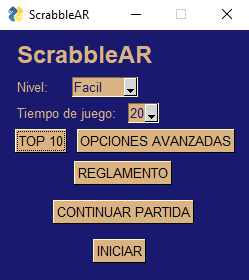
\includegraphics{images/p1.png}
\end{center}

Al iniciar una nueva, se pedirá al usuario que ingrese su nombre. Una vez ingresado el mismo, se procede a jugar. Allí se mostrará el tablero, el atril del jugador y del CPU, referencias de los casilleros según el color, puntaje total, cantidad de fichas restantes, tiempo restante y las jugadas, tanto del jugador como del CPU.

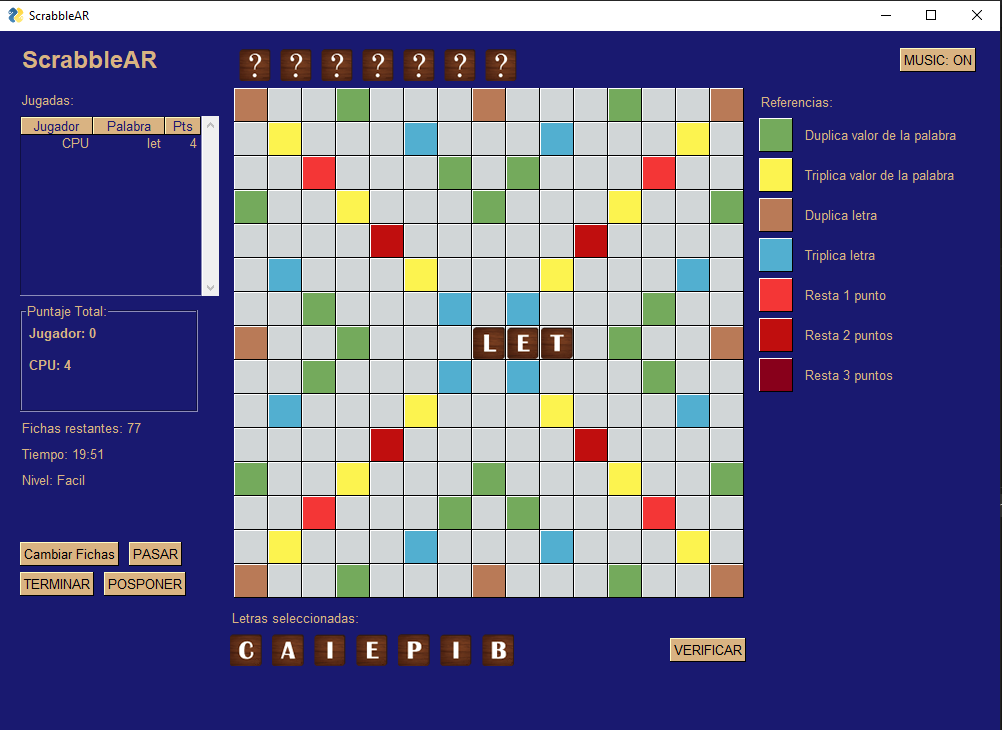
\includegraphics[width=\textwidth]{images/p2.png}

Luego la jugabilidad junto con sus reglas, se explican en la sección "Reglas" 

\hyperref[sec:reglas]{Reglas}


\section{Guía para el desarrollador}
En esta sección se explicará al programador como se plantearon las soluciones y el uso de módulos específicos.

Para comenzar, implementamos el uso de GitHub para el desarrollo del proyecto, ya que permite una mejor organización en cuanto a lo que va a trabajar cada integrante, para esto se crearon cuatro ramas, en la que una se utilizó para combinar el código en el que cada desarrollador trabajó en su rama.

En cuanto a los módulos, se utilizaron ocho de la librería estándar de Python, estos permiten por ejemplo manejo de archivos, generación de secuencias numéricas aleatorias, obtención de fechas y hora en tiempo real entre otros.

Para la interfaz gráfica, como fue antes mencionado en la sección cinco, se utilizó PySimpleGUI ya que fue la herramienta recomendada por la cátedra por su fácil implementación y optimización en la creación de interfaces gráficas.

Para la verificación de palabras se utilizó Python, ya que esta fue la recomendación de la cátedra al igual que PySimpleGUI, debido a que el mismo ofrece múltiples funcionalidades que cumplen con este propósito.

En el apartado de sonido, se utilizaron distintos módulos los cuales abarcan cada cual su tarea.

Para la música, se usó PyGame, ya que este permite reproducirla de forma asincrónica, generar una cola de reproducción, silenciar, entre otras funcionalidades.

Para los efectos de sonido, por cuestiones de compatibilidad con los sistemas operativos, decidimos usar tres módulos. En el caso de Windows, se utilizó playsound, ya que permite reproducir los sonidos de forma asincrónica, pero por restricciones del módulo, esto no se puede llevar a cabo en GNU/Linux. Por eso, en este último se utilizaron los módulos soundfile y sounddevice, los cuales si permiten esta funcionalidad. Si bien, estos módulos anteriormente mencionados funcionan tanto en GNU/Linux, como en Windows, en este último nos hemos encontrado con problemas en la reproducción del audio, por lo que optamos utilizar los módulos de la forma previamente mencionada.





\end{document}
